\hypertarget{cmd:extras-stempel}{}
\section{Stempeleditor}

\wspplot\ bietet Ihnen die M�glichkeit, neben dem \bce-Stempel auch eigene
Stempel mit ihrem Firmen- / Institutslogo bzw -layout zu integrieren. Hierzu steht ein
eigenst�ndiges Programm, der Stempeleditor, zur Verf�gung, den Sie �ber \menu{Extras / Stempeleditor}
aus dem Plotterprogramm heraus aufrufen k�nnen. Standardm��ig wird
Ihnen ein Stempel, entweder der BCE-Stempel oder der Stempel des Bayerischen
Landesamtes f�r Wasserwirtschaft mitgeliefert. Der mitgelieferte Stempel findet sich im
Plotterinstallationsverzeichnis (standardm��ig \file{C:/Programm/BCE/Wspwin/Plotter}) und hat die Endung '\file{.stp}'. Ein vorhandener Stempel kann �ber \menu{Datei / �ffnen} im Stempeleditor
ausgew�hlt werden. W�hlen Sie \menu{Datei / Neu}, wenn Sie einen neuen Stempel erzeugen
m�chten. Es sind dann zun�chst die Eigenschaften des Stempels, d.h. seine Gr��e und der
Name, �ber den der Stempel aus dem eigentlichen Plotprogramm heraus aufgerufen wird,
anzugeben (Abb. \ref{fig:stempel-eigenschaften}).

\begin{figure}[hbtp]
	\begin{center}
		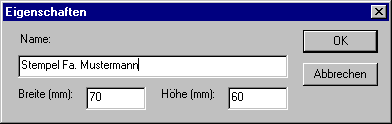
\includegraphics[scale=0.80]{stempel-eigenschaften}
	\end{center}
	\caption{Stempeleigenschaften}
	\label{fig:stempel-eigenschaften}
\end{figure}

Zur Generierung des Stempels steht eine Zeichensymbolleiste wie im eigentlichen
Plotterprogramm zur Verf�gung. Die Funktionen stehen auch im Men�punkt \menu{Zeichnen} zur
Verf�gung. Texte k�nnen nach Anklicken des A-Symbols und Aufziehen eines Textfeldes
eingegeben werden. Standardm��ig wird das Textfeld mit einem Platzhalter (z.B.
Auftraggeber) vorbesetzt. Wenn man in dem Feld einen Doppelklick ausf�hrt, gelangt man
wieder in die Attributmaske (vgl. Abb. \ref{fig:stempel-attribute}). 
In dem Listenfeld \ctrl{Typ} finden sich eine Vielzahl
von Platzhaltern, von denen man den gew�nschten selektieren kann. M�chte man keinen
Platzhalter verwenden, w�hlt man in dem Listenfeld '$<$keine$>$'. In diesem Fall kann man unter
\ctrl{Text} in dem Dialogfenster \dialog{Graphische Attribute} direkt einen beliebigen Text
eingeben. Alternativ kann man auch das Textfeld im Stempel markieren und nach Wahl des
A-Symbols in dem Feld selbst editieren. Hilfreich bei der Erstellung eines neuen Stempels
kann eine Gittereinrichtung sein. Die Gittergr��e legen Sie unter \menu{Extras / Gittereinrichtung}
fest (Abb. \ref{fig:stempel-gitter}). Hier bestimmen Sie auch �ber das Kontrollk�stchen
'An Gitter ausrichten', ob neu erstellte Objekte (Texte oder Zeichnungen) automatisch
am Gitternetz �ber einen Objektfang ausgerichtet werden sollen und so symmetrisch plaziert
werden.
�ber \menu{Bearbeiten / Neues Objekt einf�gen} k�nnen Sie wie im Plotter selbst fertige
Bilddateien einf�gen oder auf Programme mit OLE-Funktion zugreifen, Objekte erstellen und
diese in den Stempel integrieren. Auf diese Weise k�nnen Sie z.B ihr Firmenlogo integrieren.
F�r den Plotter wie auch den Stempeleditor ist zu beachten, da� s�mtliche Objekte wie Layer
aufzufassen sind, d.h. es kann vorkommen, da� das eine Objekt das andere �berdeckt. In
diesem Fall k�nnen Sie nach Markieren eines Objektes �ber \menu{Objekt / nach oben / unten setzen}
die Hierarchie der Darstellung modifizieren. Dies ist auch bei der
Darstellung verschiedener Datens�tze (z.B. fl�chige Darstellung mehrerer Wasserspiegel) im
Plotter zu beachten.

\begin{figure}[hbtp]
	\begin{center}
		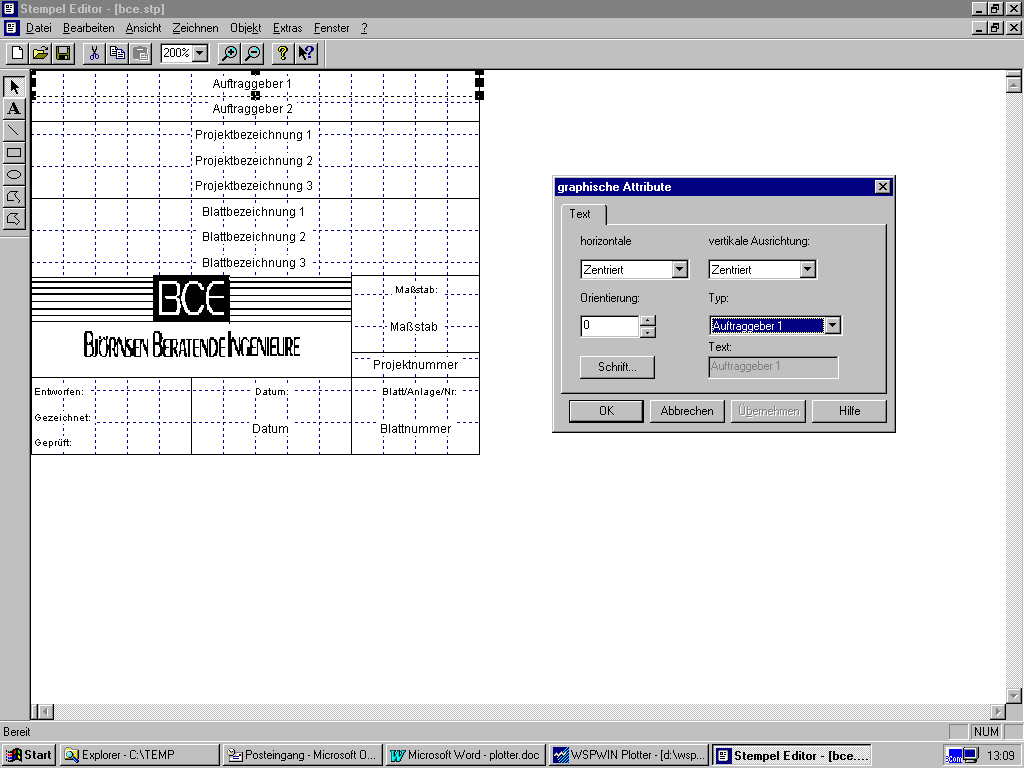
\includegraphics[scale=0.40]{stempel-attribute}
	\end{center}
	\caption{\bce-Stempel und graphische Attribute eines Textfeldes im Stempeleditor}
	\label{fig:stempel-attribute}
\end{figure}

\begin{figure}[hbtp]
	\begin{center}
		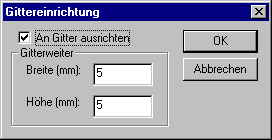
\includegraphics[scale=0.80]{stempel-gitter}
	\end{center}
	\caption{BCE-Stempel und graphische Attribute eines Textfeldes im Stempeleditor}
	\label{fig:stempel-gitter}
\end{figure}
